\setcounter{figure}{0}
\begin{questions}

\question Use disk (or washer) method to find the volume of the solid of revolution obtain by rotating the given region, $R$, about the specified axis of rotation.
\begin{parts}
\part $y=x+2$ and $y=x^2$ about the line $y=5$
  \begin{figure}[hbt!]\centering
    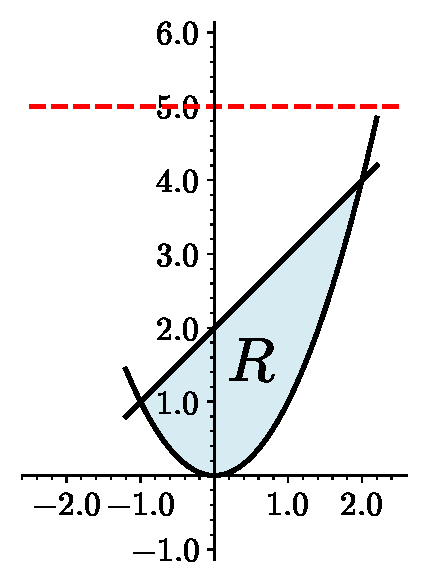
\includegraphics[scale=0.75]{plots/volume_by_slicing2_p1.pdf}
    \caption{Region between $y=x+2$ and $y=x^2$}
  \end{figure}
  
\begin{solutionorbox}[5.0in]

\end{solutionorbox}


\part $y=2$ and $y=\sqrt{x}$ about the line $x=-2$
  \begin{figure}[hbt!]\centering
    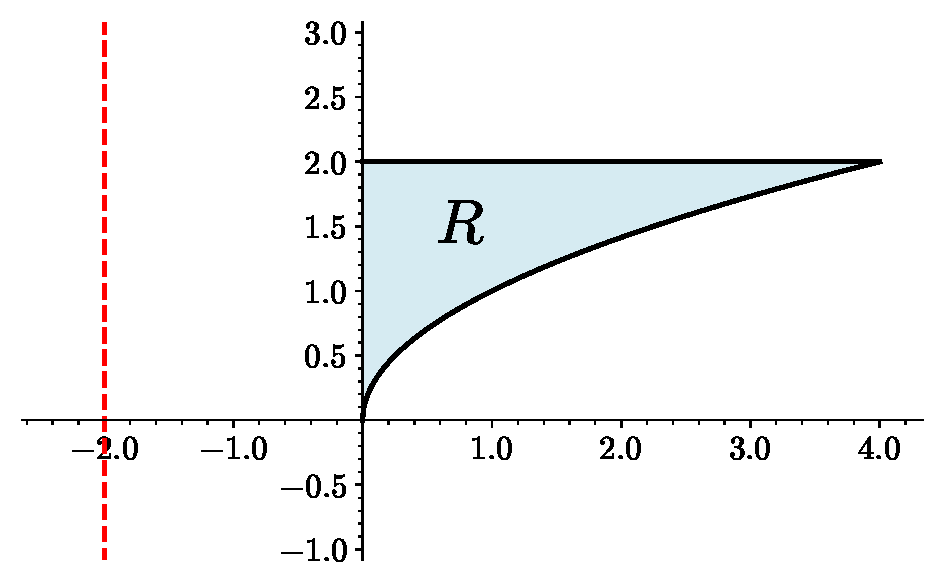
\includegraphics[scale=0.75]{plots/volume_by_slicing2_p2.pdf}
    \caption{Region between $y=2$ and $y=\sqrt{x}$}
  \end{figure}
\begin{solutionorbox}[6.0in]

\end{solutionorbox}

\end{parts}



\end{questions}